% !TeX root = index.tex

\subsection{Processor instruction set tables}\label{subsec:instruction_sets}
\arrayrulecolor{black}
\begin{longtable}[h!]{| l | p{.70\textwidth} | c |}
\caption{Instruction set for RISC processor. * Required immediate size in bytes}
\label{tab:risc_instructions}\\

\hline
\rowcolor[rgb]{0.82,0.82,0.82}
Instr. & Description & I-size *\\\hline
\endhead		

\arrayrulecolor{black}\hline
\endfoot

\multicolumn{3}{|c|}{
	\cellcolor[rgb]{0.7,0.7,1}\textit{2 register instructions}} \\\hline
\arrayrulecolor[rgb]{0.82,0.82,0.82}

MOVE & Copy value from one register to other & 0 \\\hline
ADD  & Arithmetical addition & 0 \\
SUB  & Arithmetical subtraction & 0  \\
AND  & Logical AND & 0 \\
OR   & Logical OR & 0 \\
XOR  & Logical XOR & 0 \\
MUL  & Arithmetical multiplication & 0 \\
DIV  & Arithmetical division (inc. modulo) & 0 \\


\arrayrulecolor{black}\hline
\multicolumn{3}{|c|}{
	\cellcolor[rgb]{0.7,0.7,1}\textit{1 register instructions}} \\
\hline\arrayrulecolor[rgb]{0.82,0.82,0.82}


COPY0 & Copy intimidate to a register 0 & 1 \\
COPY1 & Copy intimidate to a register 1 & 1 \\
COPY2 & Copy intimidate to a register 2 & 1 \\
COPY3 & Copy intimidate to a register 3 & 1 \\\hline

ADDC & Arithmetical addition with carry bit& 0 \\
ADDI & Arithmetical addition with immediate & 1 \\
SUBC & Arithmetical subtraction with carry bit & 0 \\
SUBI & Arithmetical subtraction with immediate & 1 \\\hline

ANDI & Logical AND with immediate & 1 \\
ORI  &  Logical OR with immediate & 1 \\
XORI &  Logical XOR with immediate & 1 \\\hline

CI0  & Replace intimidate value byte 0 for next instruction & 1 \\
CI1  & Replace intimidate value byte 1 for next instruction & 1 \\
CI2  & Replace intimidate value byte 2 for next instruction & 1 \\\hline

SLL  & Shift left logical & 1 \\
SRL  & Shift right logical & 1 \\
SRA  & Shift right arithmetical & 1 \\\hline

LWHI & Load word (high byte) & 3 \\
SWHI & Store word (high byte, reg. only) & 0 \\
LWLO & Load word (low byte) & 3 \\
SWLO & Store word (low byte, stores high byte reg.) & 3 \\\hline

INC  & Increase by 1 & 0 \\
DEC  & Decrease by 1 & 0 \\
GETAH& Get ALU high byte reg. (only for MUL \& DIV \& ROL \& ROR) & 0 \\
GETIF& Get interrupt flags & 0 \\\hline

PUSH & Push to stack & 0 \\
POP  & Pop from stack & 0 \\
COM  & Send/Receive to/from com. block & 1 \\\hline

BEQ  & Branch on equal & 3 \\
BGT  & Branch on greater than & 3 \\
BGE  & Branch on greater equal than & 3 \\
BZ   & Branch on zero & 2 \\

\arrayrulecolor{black}\hline
\multicolumn{3}{|c|}{
	\cellcolor[rgb]{0.7,0.7,1}\textit{0 register instructions}
} \\
\hline\arrayrulecolor[rgb]{0.82,0.82,0.82} 

CALL & Call function, put return to stack & 2 \\
RET  & Return from function & 0 \\
JUMP & Jump to address & 2 \\
RETI & Return from interrupt & 0 \\
INTRE& Set interrupt entry pointer & 2 \\\hline


\end{longtable}	

\arrayrulecolor{black}
\begin{longtable}[h!]{| l | p{0.8\textwidth} |}
	\caption{Instructions for OISC processor.}
	\label{tab:oisc_instructions}\\
	
	\hline 
	\rowcolor[rgb]{0.82,0.82,0.82}
	Name & Description \\\hline
	\endhead		
	
	\arrayrulecolor{black}\hline
	\endfoot
	
	\multicolumn{2}{|c|}{
		\cellcolor[rgb]{0.7,0.7,1}\textit{Destination Addresses}} \\\hline
	\arrayrulecolor[rgb]{0.82,0.82,0.82}
	
	ACC0 & Set ALU source A accumulator \\
	ACC1 & Set ALU source B accumulator \\\hline
	BR0  & Set Branch pointer register (low byte) \\
	BR1  & Set Branch pointer register (high byte) \\
	BRZ  & If source value is 0, set program counter to branch pointer \\\hline
	STACK& Push value to stack \\
	MEM0 & Set Memory pointer register (low byte) \\
	MEM1 & Set Memory pointer register (middle byte) \\
	MEM2 & Set Memory pointer register (high byte) \\
	MEMHI& Save high byte to memory at memory pointer \\
	MEMLO& Save low byte to memory at memory pointer \\\hline
	COMA & Set communication block address register \\
	COMD & Send value to communication block \\\hline
	REG0 & Set general purpose register 0 \\
	REG1 & set general purpose register 1 \\
	
	\arrayrulecolor{black}\hline
	\multicolumn{2}{|c|}{
		\cellcolor[rgb]{0.7,0.7,1}\textit{Source Addresses}} \\\hline
	\arrayrulecolor[rgb]{0.82,0.82,0.82}
	
	NULL & Get constant 0 \\
	ALU0 & Get value at ALU source A accumulator \\
	ALU1 & Get value at ALU source B accumulator \\\hline
	
	ADD  & Get Arithmetical addition of ALU sources \\
	ADDC & Get Arithmetical addition carry \\
	ADC  & Get Arithmetical addition of ALU sources and carry \\\hline
	
	SUB  & Get Arithmetical subtraction of ALU sources \\
	SUBC & Get Arithmetical subtraction carry \\
	SBC  & Get Arithmetical subtraction of ALU sources and carry \\\hline
	
	AND  & Get Logical AND of ALU sources \\
	OR   & Get Logical OR of ALU sources \\
	XOR  & Get Logical XOR of ALU sources \\\hline
	
	SLL  & Get ALU source A shifted left by source B \\
	SRL  & Get ALU source A shifted right by source B \\
	ROL  & Get rolled off value from previous SLL instance \\
	ROR  & Get rolled off value from previous SRL instance \\\hline
	
	MULLO& Get Arithmetical multiplication of ALU sources (low byte) \\
	MULHI& Get Arithmetical multiplication of ALU sources (high byte) \\
	DIV  & Get Arithmetical division of ALU sources \\
	MOD  & Get Arithmetical modulo of ALU sources \\\hline
	
	EQ   & Check if ALU source A is equal to source B \\
	GT   & Check if ALU source A is greater than source B \\
	GE   & Check if ALU source A is greater or equal to source B \\
	NE   & Check if ALU source A is not equal to source B \\
	LT   & Check if ALU source A is less than source B \\
	LE   & Check if ALU source A is less or equal to to source B \\\hline
	
	BR0  & Get Branch pointer register value (low byte) \\
	BR1  & Get Branch pointer register value (high byte) \\	
	PC0  & Get Program counter value (low byte) \\
	PC1  & Get Program counter value (high byte) \\\hline
	
	MEM0 & Get Memory pointer register value (low byte) \\
	MEM1 & Get Memory pointer register value (middle byte) \\
	MEM2 & Get Memory pointer register value (high byte) \\
	MEMHI& Load high byte from memory at memory pointer \\
	MEMLO& Load low byte from memory at memory pointer \\\hline
	
	STACK& Pop value from stack \\
	ST0  & Get stack address value (low byte) \\
	ST1  & Get stack address value (high byte) \\
	
	COMA & Get communication block address register value \\
	COMD & Read value from communication block \\\hline
	
	REG0 & Get value from general purpose register 0 \\
	REG1 & Get value from general purpose register 1 \\
	
\end{longtable}	
\pagebreak
\subsection{Glossary}\label{subsec:glossary}
\textbf{CISC (Comprex Instruction Set Computer)} refers to a computer architecture that follows philosophy of implementing many instructions that can process complex functions.\\
\textbf{RISC (Reduced Instruction Set Computer)} refers to a computer architecture that follows philosophy of keeping fewer common instructions and execute complex functions in software. In this report it is commonly used to refer to the developed RISC processor.\\
\textbf{OISC (One Instruction Set Computer)} computer architecture that has only a single instruction. As know as Ultimate RISC. In this report it is commonly used to refer to the developed OISC processor.\\
\textbf{TTA (Transport Triggered Architecture)} type of processor that does not have control block and data is directly control by the internal transport buses.\\
\textbf{VLIW (Very Long Instruction Word)} refers to instructions set that encodes multiple parallel operations into a single instruction.\\
\textbf{MIPS (Microprocessor without Interlocked Pipelined Stages)} is a specific RISC architecture developed by MIPS Technologies, Inc.\\
\textbf{ALU (Arithmetic Logic Unit)} processor part that is responsible for the mathematical operations performed upon data.\\
\textbf{RAM (Random Access Memory)} refers so dynamic volatile processor memory.\\
\textbf{ROM (Read Only Memory)} refers to memory that stores program instructions.\\
\textbf{FPGA (Field Programmable Gate Array)} a chip or device that can be configured to have any digital circuit within its limits.\\
\textbf{HDL (Hardware Description Language)} Language used to code digital circuit behaviour. SystemVerilog specifically was used throughout this project.\\
\textbf{PLL (Phase-Locked Loop)} a control system and a circuit which is commonly used to control singal phase, frequency, duty cycle and other parameters.\\
\textbf{Architecture} refers to processor functioning principles, general operation and its instruction set.\\
\textbf{Microarchitecture} refers to digital logic that is used to implement a computer architecture.

\pagebreak
\subsection{Unconventional diagram notation}\label{subsec:notation}
This is a short explanation of unconventional digital logic notation and symbols used in this report diagrams. Note that notations in diagram are only to represents logical operation and not how it is implemented on circuit level. This means that an adder symbol may be implemented either as ripple carry or carry look ahead adder.

\begin{figure*}[bh]
	\centering
	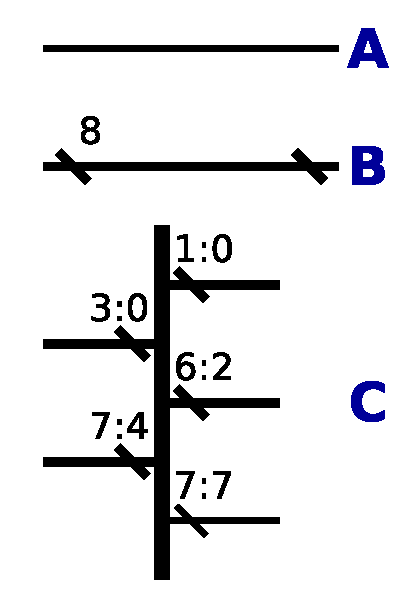
\includegraphics[scale=0.4]{../resources/symbols/wires.eps}
	\caption{(A) represents a single connecting wire; (B) represents a bus with width of 8; (C) represents a bus branching. Left side connects two 4 bit buses at indexes 0-3 and 4-7. Right side connects two buses, 2bit and 5bit viewing from top to bottom and a single wire that takes index 7.}
	\vspace{1cm}
	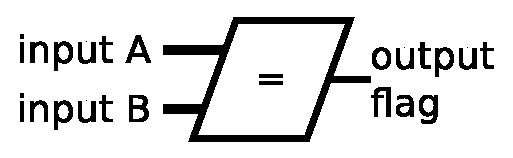
\includegraphics[scale=0.4]{../resources/symbols/eq.eps}
	\caption{This represents an equality operation. It sets output flag to high of both input bus values are equal.}
	\vspace{1cm}
	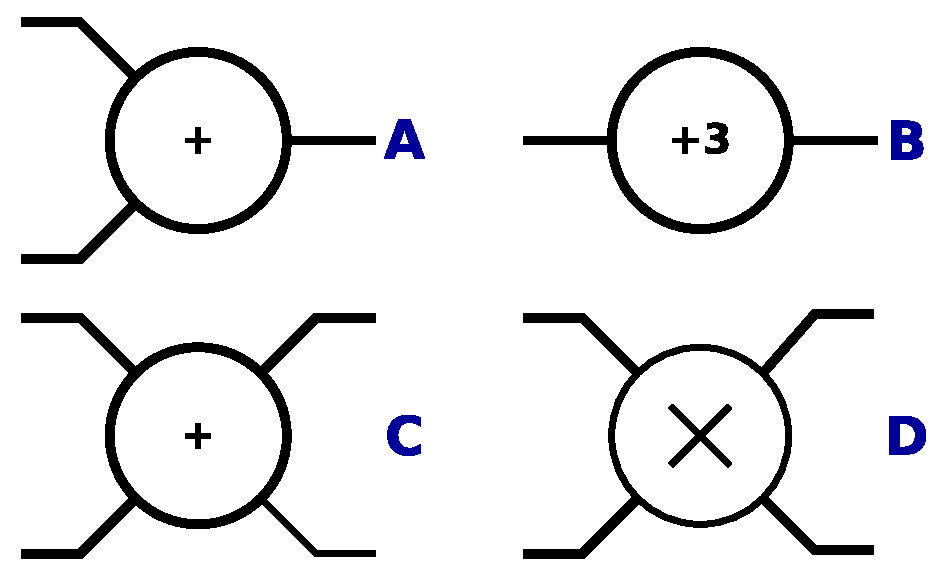
\includegraphics[scale=0.4]{../resources/symbols/ops.eps}
	\caption{(A) represents an adder that takes two inputs from left side and output results to bus on the right; (B) represents adder with a single input being a constant shown as decimal number in the centre of symbol; (C) repesents same adder as A, except with carry out flag at the right bottom; (D) represents multiplication circuit with two inputs at the left and two outputs at the right. As multiplication produces twice the width result than input, top output is higher word and bottom output is lower word.}
\end{figure*}



